\documentclass[journal]{IEEEtran}
\usepackage{graphics}
\usepackage{algorithm}
\usepackage{algpseudocode}
\usepackage{listings}
\usepackage{float}

\begin{document}


\title{Implementation of a Carry Lookahead Fast Adder}
\author{
	Healy, Matthew
	\texttt{mhealy@mst.edu}\\
	\and
	Johnston, Jaxson
	\texttt{jnjt37@mst.edu}\\
	\and
	Grbe\`sa, Lukas
	\texttt{lgqq3@mst.edu}\
}

\maketitle


\begin{abstract}
Carry lookahead adders are one of the most common fast-adder architectures
used in high performance computing to date. They allow for arbitrarily large
summations with only $O(log(n))$ complexity, rather than the $O(n)$ complexity
of a traditional ripple-carry adder.

The purpose of this project is to implement a simulation of the execution
of a carry lookahead adder using the Intel 8051 architecture. Although this
simulation cannot achieve the performance of a hardware implementation, it
serves as a proof of concept for a carry lookahead adder.

\end{abstract}

\section{Introduction}\label{sec:intro}
The carry lookahead adder was originally patented by IBM\cite{patent} in 1972.
As time passed and technology improved, this method of addition was shown
to be even more useful than originally thought, as it allows for the quick
computation of numbers that would take a non-insignificant amount of time
using the traditional ripple-carry method.

Our goal in this project is to implement a simulation of a carry lookahead
adder on the 8051 microcontroller as a proof of concept. Since execution is
serial, this simulation will not be faster than the built-in adding operations,
as we are unable to calculate multiple things at once, as we could were we
building a hardware model of a carry lookahead adder.

\section{Approach}\label{sec:approach}
The carry value of a certain bit addition
can be determined by looking at the previous
pair of bits, finding their generate and propagate values, and comparing the
propagate value to the carry of the previous bit operation. After a string of
carries is created then all that must be done is two XOR operations because
XORing the first input with the second input and XORing the result of that
operation with the carry string gives the logical equivalent of adding the two
numbers directly.

There are only two registers in the 8051($R0$ and $R1$) that can be used with
indirect addressing. This means that we could only have two pointers to our data
at a time. Since we planned on having up to five strings of stored
data($A, B, P, G,$ and Carry), we know that we had to reuse memory. To solve this,
we had $P$ replace input $A$ and $G$ replace input $B$ in memory, and then had the
carry string overwrite each bit of the generate string one by one. We knew this
was a workable solution, since only the carry depends on the $G$ string, and the
final sum depends only on the $P$ string and the carry string.

Since bitwise operations could only be performed on the carry bit and a single
bit of either the $A$ register or the $B$ register, and only the $A$ register
can be rotated(which was necessary for our generation of the carry string,
which can be seen in the included source code), we were forced to constantly
move data from the $A$ register into memory as temporary storage, while the $B$
register was moved to $A$ for rotation. In hindsight, this could have been
accomplished much more easily with a simple \texxttt{SWAP} command, but we did
not feel that the performance increase such a change would provide was worth the
additional effort of a refactor.

Since we needed to include the total number of cycles that our operation took
to complete, we needed to start and stop a timer before and after the operation,
respectively. Timer mode 1 was chosen, as it was 16 bit, and so could run for
the longest amount of time without overflowing. This choice was not arbitrary,
as any timer that would overflow would cause us to need to check for timer
overflow after every instruction, and increment some form of counter to account
for the wraparound. This would have also added instructions(and so cycles)
to our program that were completely useless for the actual addition. We ensured
that our timer never overflowed during our tests, which included the largest
input size we could account for, by checking the value of the $TF1$ flag at the
end of execution. Since it was never set, we assumed it safe to just let the
timer run unmolested until the end of execution, and then read the $TH1$ and
$TL1$ bytes to see the total time elapsed.

We chose a fixed-baudrate serial mode, since doing any form of variable
baudrate would require the use of another timer, and unnecessarily complicate
the program further.

\section{Results and Discussion}\label{sec:discuss}

By first generating our Propogate($P$) and Generate($G$) strings from the input,
and then stepping through our carry string and deriving each bit from the
$P$ and $G$ strings and the previous carry bit, we emulate the stages of
operation of a carry lookahead adder.

The $P$ string is created by XORing each pair of respective input bits, and the
$G$ by ANDing together each pair of input bits. This would be done in hardware
with blocks of two logic gates all operating in parallel, and would take
approximately $2\Delta t$ to complete.

The next stage, wherein the $P$ and carry bit are XORed together to create the
sum, is emulated by a loop that XORs bytes of the carry string with bytes of
the $P$ string. While this adds another n time in the software solution, it
would implement only another $2\Delta t$ in a hardware solution, since it would
bo only two more logic gates for each bit, all operating in parallel.

Algorithm \ref{alg:pseudo}
shows the basic implementation of this simulation:
\begin{algorithm}[H]
\caption{Pseudocode for CLA Adder}
\label{alg:pseudo}
\begin{algorithmic}
\State R3 $\rightarrow$ carry string
\State R6 $\rightarrow$ Input A
\State R7 $\rightarrow$ Input B

\ForAll{bytes $P_i\in P, G_i\in G, RX_i\in RX$}
	\State $P \gets R6 \oplus R7$
	\State $G \gets R6 \land R7$
\EndFor
\ForAll{bits $C_i\in C, P_i\in P, G_i\in G$}
	\State $C \gets G \lor (P \land C)$
\EndFor

\ForAll{bytes $SUM_i\in SUM, C_i\in C, P_i\in P$}
	\State $SUM_i \gets C_i \oplus P_i$
\EndFor
\end{algorithmic}
\end{algorithm}

\begin{table}[H]
	\caption{Inputs, Sum, and Computation time}
	\label{tab:time}
	\resizebox{3.5in}{!}{
	\begin{tabular}{|r|r|l|l|}
		\hline
		\textbf{Operand 1} & \textbf{Operand 2} & \textbf{Sum} & \textbf{Time(clock pulses)}\\
		\hline
		$0x8A$ & $0x25$ & $0xAF$ & $0xA0$\\
		\hline
		$0x1FFF$ & $0xA222$ & $0xC111$ & $0x12E$\\
		\hline
		$0x3EFF$ & $0x8AAA$ & $0xC9A9$ & $0x12E$\\
		\hline
		$0x254621$ & $0xAAAAAA$ & $0xCFF0CB$ & $0x01D4$\\
		\hline
		$0x8532AA$ & $0x243699$ & $0xA96943$ & $0x01D5$\\
		\hline
		$0x23456789$ & $0x98765432$ & $0xBBBBBBBB$ & $0x026A$\\
		\hline
		$0xABABABAB$ & $0x11111111$ & $0xBCBCBCBC$ & $0x04C2$\\
		\hline
		$0xC1C1C1C1C1$ & $0x1C1C1C1C1C$ & $0xDDDDDDDDDD$ & $0x0300$\\
		\hline
		$0x123456789ABC$ & $0x123456789ABC$ & $0x2468ACF13578$ & $0x0396$\\
		\hline
		$0x1234567C1C1C1C$ & $0x11AAAAAA8532AA$ & $0x23DF0126A14EC6$ & $0x042E$\\
		\hline
	\end{tabular}}
\end{table}

\begin{figure}[H]
	\resizebox{3.5in}{!}{
	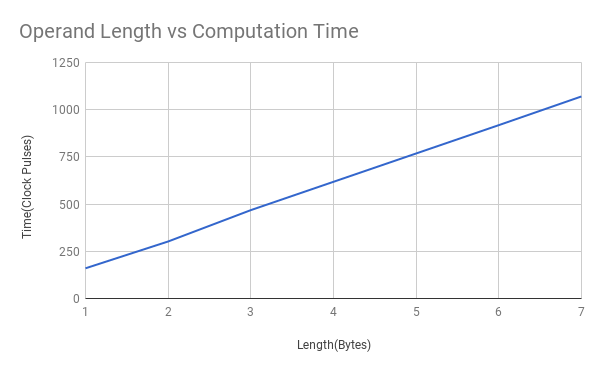
\includegraphics{chart.png}}
	\caption{Inputs vs Computation Time}
	\label{fig:chart}
\end{figure}

As can be seen in Fig. \ref{fig:chart}, this software simulation falls far
short of the speed of its hardware implementation. However, it does match very
closely the speed of a ripple-carry add on the 8051 microcontroller, changing
only the constant in the time-complexity.

\section{Summary and Conclusion}

Upon testing we found that because the carry lookahead adder must be
executed in serial, the simulation doesn't end up being any faster than simply
adding the two values together. With that said, we were still successful in
creating and implementing the carry lookahead adder, and, if given access to
different hardware, we would be able to lower the execution time for the
addition.

\section{Source Code}\label{sec:code}

\lstinputlisting[firstline=13, basicstyle=\tiny]
{fast_addr.asm}

\begin{thebibliography}{99}

\bibitem{patent}
  Franz, S. and Dieter, S.
  Parallel binary carry look-ahead adder system.
  [US Patent 3,700,875].
  \\\texttt{https://www.google.com/patents/US3700875}
  1972.
}


\end{thebibliography}
\end{document}
